\section{Transformations of Functions} \label{S:0.3.Transformations}


\vspace*{-14 pt}
\framebox{\hspace*{3 pt}
\parbox{6.25 in}{\begin{goals}
\item How can new functions be generated by shifts, stretches, and transformations of
    well-known functions?
\item How can we mathematically describe symmetric functions?
\item How can we build inverse functions, and when do those functions exist?
\end{goals}} \hspace*{3 pt}}


\begin{web}
\item
    \href{https://www.khanacademy.org/math/algebra2/functions_and_graphs/shifting-reflecting-functions/v/shifting-and-reflecting-functions}{Khan
    Playlist: Shifting and reflecting functions}
\item
    \href{https://www.khanacademy.org/math/algebra2/functions_and_graphs/analyzing_functions}{Khan
    Playlist: Analyzing functions}
\item
    \href{http://www.geogebratube.org/student/m93018}{Geogebra Applet for function
    transformations}
\end{web}

\nin \hrulefill


\subsection*{Introduction}
There are infinitely many functions that can be generated using the basic mathematical
operations (addition, subtraction, multiplication, division, and exponentiation) along
with {\it simple} functions such as roots, exponentials, and trigonometric functions.  In
fact, we can build entire families of functions based only on these simple building
blocks.

\begin{pa} \label{PA:0.3}
The goal of this activity is to explore and experiment with the function
\[ F(x) = Af(B(x-C))+D. \]
The values of $A$, $B$, $C$, and $D$ are constants and the function $f(x)$ will be
henceforth called the {\it parent function}.  To facilitate this exploration, use the
applet located at \\
\href{http://www.geogebratube.org/student/m93018}{http://www.geogebratube.org/student/m93018}.
\ba
    \item Let's start with a simple function.  Let the parent function be $f(x) = x^2$.
        \bei
            \item Fix $B=1$, $C=0$, and $D=0$.  Write a sentence or two describing the
                action of $A$ on the function $F(x)$.
            \item Fix $A=1$, $B=1$, and $D=0$.  Write a sentence of two describing the
                action of $C$ on the function $F(x)$.
            \item Fix $A=1$, $B=1$, and $C=0$.  Write a sentence of two describing the
                action of $D$ on the function $F(x)$.
            \item Fix $A=1$, $C=0$, and $D=0$.  Write a sentence of two describing the
                action of $B$ on the function $F(x)$.
        \eei
    \item Test your conjectures with the functions $f(x) = |x|$ (typed \texttt{abs(x)}),
        $f(x) = x^3$, $f(x) = \sin(x)$, $f(x) = e^x$ (typed \texttt{exp(x)}), and any
        other function you find interesting. 
\ea
\end{pa} \afterpa


% Your preview activity goes here

\subsection*{Function Transformations}
In Preview Activity \ref{PA:0.3} we experimented with the four main types of function
transformations.  You no doubt noticed that the values of $C$ and $D$ {\it shift} the
parent function and the values of $A$ and $B$ {\it stretch} the parent function.  More
descriptively, if $f(x)$ is a parent function and 
\[ F(x) = Af(B(x-C))+D \] 
then the actions of each parameter are described in Table \ref{tab:0.3.trans}.
\begin{table}[h!]
    \centering
    \begin{tabular}{|c|l|}
        \hline
        Parameter & Action \\ \hline \hline
        $A$ & Stretch the parent function vertically \\
        $B$ & Stretch the parent function horizontally \\
        $C$ & Shift the parent function horizontally \\
        $D$ & Shift the parent function vertically \\ \hline
    \end{tabular}
    \caption{Actions of stretch- and shift-type transformations}
    \label{tab:0.3.trans}
\end{table}


\bex
Consider the function $f(x)$ in the left-hand plot of Figure \ref{F:0.3.Ex1}.  Plot $2f(x)$, $f(x)+1$,
$f(x-1)$, and $f(2x)$.
\eex
\def\scl{0.75}
\begin{figure}[ht!]
    \begin{center}
        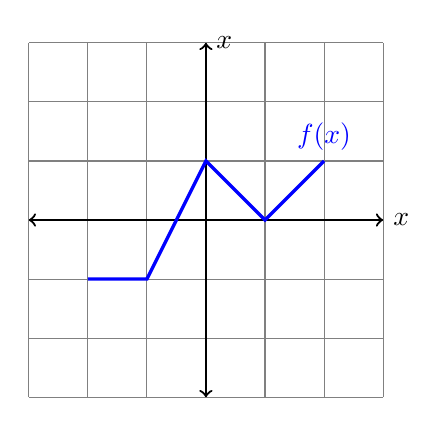
\begin{tikzpicture}[scale=\scl]
            \draw[color=gray] (-3,-3) grid (3,3);
            \draw[thick, black, <->] (-3,0) -- (3,0) node[anchor=west]{$x$};
            \draw[thick, black, <->] (0,-3) -- (0,3) node[anchor=west]{$x$};
            \draw[very thick, blue] (-2,-1) -- (-1,-1) -- (0,1) -- (1,0) -- (2,1)
            node[anchor=south]{$f(x)$}; 
        \end{tikzpicture} 
        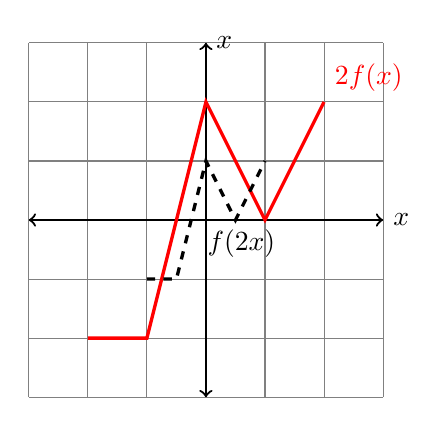
\begin{tikzpicture}[scale=\scl]
            \draw[color=gray] (-3,-3) grid (3,3);
            \draw[thick, black, <->] (-3,0) -- (3,0) node[anchor=west]{$x$};
            \draw[thick, black, <->] (0,-3) -- (0,3) node[anchor=west]{$x$};
            \draw[very thick, red] (-2,-2) -- (-1,-2) -- (0,2) -- (1,0) -- (2,2)
            node[anchor=south west]{$2f(x)$}; 
            \draw[very thick, black, dashed] (-1,-1) -- (-0.5,-1) --
            (0,1) -- (0.5,0) -- (1,1); 
            \draw[black] (0.6,0) node[anchor=north]{$f(2x)$};
        \end{tikzpicture}
        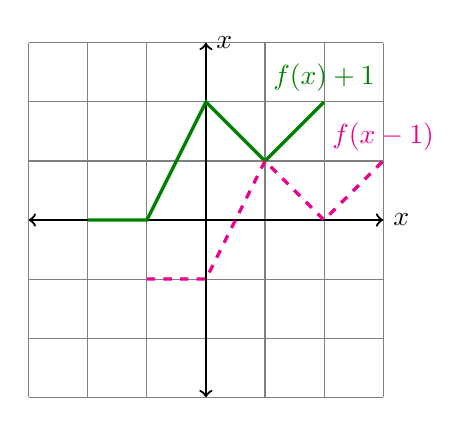
\begin{tikzpicture}[scale=\scl]
            \draw[color=gray] (-3,-3) grid (3,3);
            \draw[thick, black, <->] (-3,0) -- (3,0) node[anchor=west]{$x$};
            \draw[thick, black, <->] (0,-3) -- (0,3) node[anchor=west]{$x$};
            \draw[very thick, green!50!black] (-2,0) -- (-1,0) -- (0,2) -- (1,1) -- (2,2)
            node[anchor=south]{$f(x)+1$}; 
            \draw[very thick, magenta, dashed] (-1,-1) -- (0,-1) -- (1,1) -- (2,0) -- (3,1)
            node[anchor=south]{$f(x-1)$}; 
        \end{tikzpicture}
    \end{center}
    \caption{A function with transformations.}
    \label{F:0.3.Ex1}
\end{figure}
You should notice the following features of these solutions:
\begin{itemize}
    \item In $g(x)=2f(x)$, the ``2'' simply doubled all of the $y$-values from $f(x)$.  
    \item In $j(x)=f(2x)$, the ``2'' actually cut all of the $x$-values in half from $f(x)$.
        This is potentially contrary to what you might expect. Verify this by substituting
        values in for $x$.
    \item In $h(x)=f(x)+1$, the ``+1'' simply adds 1 unit to all of the $y$-values from
        $f(x)$.
    \item In $k(x)=f(x-1)$, the ``-1'' actually moves the graph of $f(x)$ to the right.
        This is potentially contrary to what you might expect. Verify this by substituting
        values in for $x$.
\end{itemize}
\afterex


\begin{activity}\label{A:0.3.1}
    Consider the function $f(x)$ displayed in Figure \ref{F:0.3.Act1}.
    \ba
        \item Plot $g(x) = -f(x)$ and $h(x) = f(x)-1$.
        \item Define the function $k(x) = -f(x)-1$.  Does it matter which order you
            complete the tranformations from part (a) to result in $k(x)$?  Plot the
            functions resulting from doing the two transformation in part (a) in opposite
            orders.  Which of these functions is $k(x)$?
    \ea
    \begin{figure}[h!]
        \begin{center}
%             \begin{tikzpicture}[scale=0.75]
%                 \draw[color=gray] (-3,-3) grid (3,3);
%                 \draw[thick, black, <->] (-3,0) -- (3,0) node[anchor=west]{$x$};
%                 \draw[thick, black, <->] (0,-3) -- (0,3) node[anchor=west]{$y$};
%                 \draw[very thick, blue] (-2,1) -- (-1,-2) -- (0,-2) -- (1,1) -- (2,-1)
%                 node[anchor=north]{$f(x)$}; 
%             \end{tikzpicture}
%             \begin{tikzpicture}[scale=0.75]
%                 \draw[color=gray] (-3,-3) grid (3,3);
%                 \draw[thick, black, <->] (-3,0) -- (3,0) node[anchor=west]{$x$};
%                 \draw[thick, black, <->] (0,-3) -- (0,3) node[anchor=west]{$y$};
%             \end{tikzpicture}
            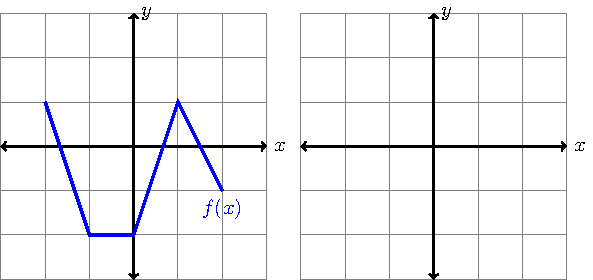
\includegraphics[width=0.65\columnwidth]{figures/0-3-fig2.pdf}
        \end{center}
        \caption{Function transformation for Activity \ref{A:0.3.1}} \label{F:0.3.Act1}
    \end{figure}
\end{activity}
\begin{smallhint}
    \ba
        \item Think of the ``$-$'' in front of $f(x)$ as a $-1$.  What is the difference
            between multiplying by $-1$ and adding $-1$?
        \item Think about the order of mathematical operations.
    \ea
\end{smallhint}
\begin{bighint}
    \ba
        \item $g(x)$ should be a vertical stretch and $h(x)$ should be a vertical shift.
        \item A very methodical way to approach this problem would be to choose several
            particular $x$ values and follow the order of operations to determine the
            output for $k$.
    \ea
\end{bighint}
\begin{activitySolution}
    \ba
        \item The function $g(x)$ should change the sign on all of the $y$ values of $f$.
            The function $h(x)$ will shift all of the $y$ values of $f$ down 1 unit.
        \item The order in which you do the transformations does matter.  In this problem
            the order of operations should be to change the sign on the $y$ value and then
            to shift 1 unit down.
    \ea
    \begin{center}
        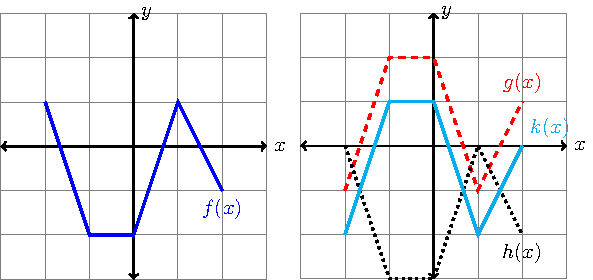
\includegraphics[width=0.65\columnwidth]{figures/0-3-fig2soln.pdf}
    \end{center}
\end{activitySolution}

\aftera




\subsection*{Composition of Functions}
When multiple transformations are applied in sequence, like in Activity \ref{A:0.3.1}, the
resulting function is actually the {\bf composition} of function transformations.  The
concept of a composition encompasses more than just transformations though.  If $f(x)$ and
$g(x)$ are functions where the range of $g(x)$ is a subset of the domain of $f(x)$ we can
form a new function $h(x) = f(g(x))$. This literally means that you are substituting
$g(x)$ in for every instance of the variable $x$ in $f(x)$.  For example, if $f(x) = x^2$
and $g(x) = e^x$ then $h(x) = f(g(x)) = \left( e^x \right)^2$ and $k(x) = g(f(x)) =
e^{(x^2)}$.  

\bex
If $f(x) = x^2$ and $g(x) = x-1$ then find $f(g(3))$, $g(f(3))$, $f(g(x))$, and
$g(f(x))$.
\eex
To evaluate $f(g(3))$ we consider that $g(3) = 2$ and $g(2) = 4$.  Therefore, $f(g(3))=4$.
Similarly, $g(f(3)) = g(9) = 8$.  The function compositions $f(g(x))$ and $g(f(x))$ are
$f(g(x)) = (x-1)^2$ and $g(f(x))=x^2 - 1$.  Notice the difference between these resulting
functions; the order that the composition takes places matters!
\afterex

\subsection*{Symmetry}
There are many ways that a function can be symmetric, but two important symmetries are (1)
reflective symmetry over the $y$-axis, and (2) $180^\circ$ rotational symmetry about the
origin.  A function that has reflective symmetry over the $y$-axis is called an {\bf even
function} and a function with rotational symmetry about the origin is called an {\bf odd
function}.  The reasoning for these names will be evident after completing Activity
\ref{A:0.3.2}.

\begin{activity}\label{A:0.3.2}
    \ba
        \item Based on symmetry alone, is $f(x) = x^2$ an even or an odd function?
        \item Based on symmetry alone, is $g(x) = x^3$ an even or an odd function?
        \item Find $f(-x)$ and $g(-x)$ and make conjectures to complete these sentences:
            \begin{itemize}
                \item If a function $f(x)$ is \underline{even} then $f(-x) =
                    $\underline{\hspace{1in}}.
                \item If a function $f(x)$ is \underline{odd} then $f(-x) =
                    $\underline{\hspace{1in}}.
            \end{itemize}
            Explain why the composition $f(-x)$ is a good test for symmetry of a function.
        \item Classify each of the following functions as even, odd, or neither.
            \[ h(x) = \frac{1}{x}, \quad j(x) = e^x, \quad k(x) = x^2-x^4, \quad n(x) =
            x^3+x^2. \]
        \item For the figure below shows only half of the function $f(x)$.  Draw the left
            half so $f(x)$ is even.  Draw the left half so $f(x)$ is odd. Draw the left
            half so $f(x)$ is neither even nor odd.
            \begin{center}
                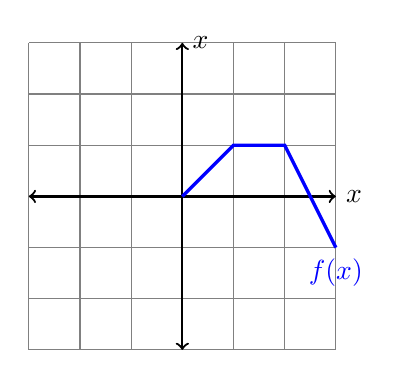
\begin{tikzpicture}[scale=0.65]
                    \draw[color=gray] (-3,-3) grid (3,3);
                    \draw[thick, black, <->] (-3,0) -- (3,0) node[anchor=west]{$x$};
                    \draw[thick, black, <->] (0,-3) -- (0,3) node[anchor=west]{$x$};
                    \draw[very thick, blue] (0,0) -- (1,1) -- (2,1) -- (3,-1)
                    node[anchor=north]{$f(x)$}; 
                \end{tikzpicture}
                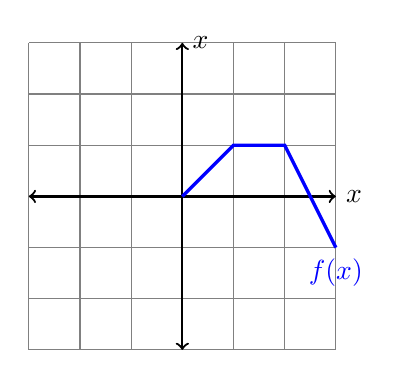
\begin{tikzpicture}[scale=0.65]
                    \draw[color=gray] (-3,-3) grid (3,3);
                    \draw[thick, black, <->] (-3,0) -- (3,0) node[anchor=west]{$x$};
                    \draw[thick, black, <->] (0,-3) -- (0,3) node[anchor=west]{$x$};
                    \draw[very thick, blue] (0,0) -- (1,1) -- (2,1) -- (3,-1)
                    node[anchor=north]{$f(x)$}; 
                \end{tikzpicture}
                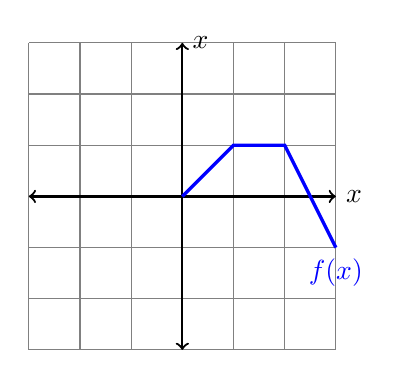
\begin{tikzpicture}[scale=0.65]
                    \draw[color=gray] (-3,-3) grid (3,3);
                    \draw[thick, black, <->] (-3,0) -- (3,0) node[anchor=west]{$x$};
                    \draw[thick, black, <->] (0,-3) -- (0,3) node[anchor=west]{$x$};
                    \draw[very thick, blue] (0,0) -- (1,1) -- (2,1) -- (3,-1)
                    node[anchor=north]{$f(x)$}; 
                \end{tikzpicture}
            \end{center}
    \ea
\end{activity}\aftera


\subsection*{Inverse Functions}
We conclude this section by discussing an important question:  If we know the action of a
function is it possible to undo that action? This question can be rephrased by saying: If
we know the output of a function can we tell exactly what the input was?  The answer to
these questions is that it depends on the type of function.  

Consider, for example, the function $f(x) = x^2$.  If we know that $f(a) = 4$ do we the
value of $a$?  Of course not!  It is obvious that $f(2) = f(-2) = 4$, so just by knowing
the output of the function $f(x) = x^2$ we cannot invert the function and find the input.
What about the function $g(x) = x^3$?  If we know that $g(b) = 8$ then there is only one
unique value of $b$, $b=2$, such that $g(b) = 8$.  Therefore it seems like we can invert
the cubic function.  

The act of {\it reversing the action of a function} can be explored geometrically.
Indeed, in Figure \ref{fig:0.3.inv} we see that if we can simply switch the values of $x$
and $y$ we will get a plot that shows how to undo the action of a function. Geometrically,
switching the role of the $x$ and the $y$ in the function is the same as reflecting over
the line $y=x$.
\begin{figure}[h!]
    \begin{center}
        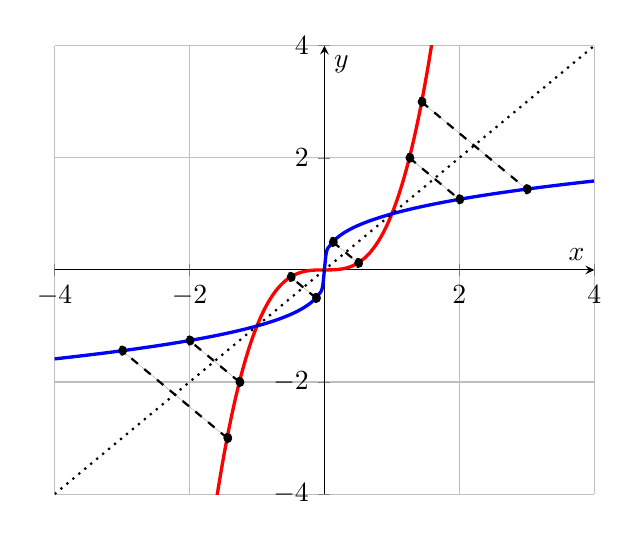
\begin{tikzpicture}
            \begin{axis}[axis lines=center, xlabel={$x$}, ylabel={$y$}, domain=-4:4,
                ymin=-4, ymax=4, xmin=-4, xmax=4, grid]
                \addplot[smooth, very thick, red, samples=150] {x^3};
                \addplot[smooth, very thick, blue, samples=150] {(x/abs(x))*abs(x)^(1/3)};
                \draw[dashed, thick, fill=black] (axis cs:1.26,2) circle(0.05cm) -- (axis
                cs:2,1.26) circle(0.05cm);
                \draw[dashed, thick, fill=black] (axis cs:-1.26,-2) circle(0.05cm) -- (axis
                cs:-2,-1.26) circle(0.05cm);
                \draw[dashed, thick, fill=black] (axis cs:-0.125,-.5) circle(0.05cm) -- (axis
                cs:-0.5,-0.125) circle(0.05cm);
                \draw[dashed, thick, fill=black] (axis cs:0.125,.5) circle(0.05cm) -- (axis
                cs:0.5,0.125) circle(0.05cm);
                \draw[dashed, thick, fill=black] (axis cs:1.44,3) circle(0.05cm) -- (axis
                cs:3,1.44) circle(0.05cm);
                \draw[dashed, thick, fill=black] (axis cs:-1.44,-3) circle(0.05cm) -- (axis
                cs:-3,-1.44) circle(0.05cm);
                \addplot[smooth, black, dotted, thick] {x};
            \end{axis}
        \end{tikzpicture}
    \end{center}
    \caption{Inverse functions. If $(x,y)$ is on one end of one of the dashed segments,
    then $(y,x)$ is on the other side.}
    \label{fig:0.3.inv}
\end{figure}

The question that remains is when an inverse function actually exists.  This is the same
as asking: ``if I reflect over $y=x$ is the end result a function?''  The answer to this
question is certain ``no'' if the function is $f(x) = x^2$ (as seen in the left-hand plot
of Figure \ref{fig:0.3.inv2}), but if we restrict the domain on $f(x) = x^2$ to $0 \le x < \infty$ then
the result is a function (as seen in the right-hand plot of Figure \ref{fig:0.3.inv2}).
This leads us to the following results:
\begin{itemize}
    \item If a horizontal line passes through a function only once, then it has a unique
        inverse found by interchanging the $x$ and the $y$.
    \item The inverse of a function can be found geometrically by reflecting the graph of
        the function over the line $y=x$.
\end{itemize}
\begin{figure}[ht!]
    \begin{center}
        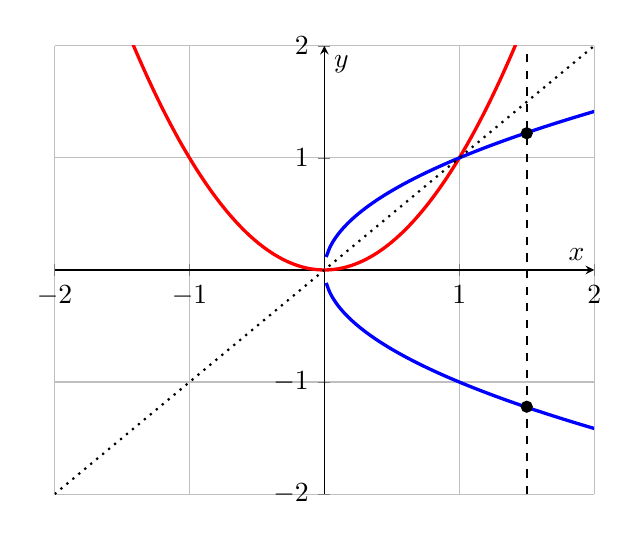
\begin{tikzpicture}
            \begin{axis}[axis lines=center, xlabel={$x$}, ylabel={$y$}, domain=-2:2,
                ymin=-2, ymax=2, xmin=-2, xmax=2, grid]
                \addplot[smooth, very thick, red, samples=150] {x^2};
                \addplot[smooth, very thick, blue, samples=150] {sqrt(x)};
                \addplot[smooth, very thick, blue, samples=150] {-sqrt(x)};
                \addplot[smooth, black, dotted, thick] {x};
                \draw[black, dashed, thick] (axis cs:1.5,-2) -- (axis cs:1.5,2);
                \draw[fill=black] (axis cs:1.5,1.22) circle(0.07cm);
                \draw[fill=black] (axis cs:1.5,-1.22) circle(0.07cm);
            \end{axis}
        \end{tikzpicture}
        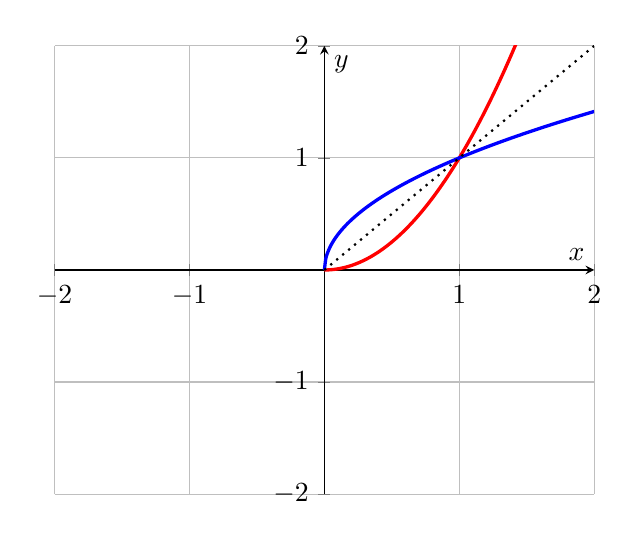
\begin{tikzpicture}
            \begin{axis}[axis lines=center, xlabel={$x$}, ylabel={$y$}, domain=0:2,
                ymin=-2, ymax=2, xmin=-2, xmax=2, grid]
                \addplot[smooth, very thick, red, samples=200] {x^2};
                \addplot[smooth, very thick, blue, samples=200] {sqrt(x)};
                \addplot[smooth, black, dotted, thick] {x};
            \end{axis}
        \end{tikzpicture}
    \end{center}
    \caption{The left-hand plot shows that after reflecting $f(x)=x^2$ across $y=x$ the
    result is not a function.  The right-hand plot shows that under a restriction of the
domain the result can be a function.}
    \label{fig:0.3.inv2}
\end{figure}

\bex
Find the inverse of the following functions.  If necessary, restrict the domain on the
function so that the inverse exists.
\ba
    \item $f(x) = x^2+1$
    \item $g(x) = ax+b$
    \item $h(x) = (2x+8)^3$
\ea
\eex
\ba
    \item To find the inverse of $f(x)$ we first interchange the $x$ and $y$.  Then we
        solve for $y$.  That is:
        \[ \text{Solve for $y$: } x = y^2+1 \quad \implies \quad y = \pm\sqrt{x-1}. \]
        Obviously the resulting solution is two equations.  By convention we choose the
        positive square root and note that the inverse only makes sense if $x\ge 1$.
        Hence, in order for the inverse to make sense we need a restriction on the domain
        of $f(x)$: If $0 \le x < \infty$ then any horizontal line only crosses the  graph
        of $f(x)$ once, and hence the inverse exists and is unique.
        \[ f^{-1}(x) = \sqrt{x-1}, \quad x \ge 1 \]
    \item Interchanging the $x$ and $y$ in this equation gives
        \[ \text{Solve for $y$: } x = ay+b \quad \implies \quad y = \frac{x-b}{a}. \]
        There is no need to restrict the domain of $g(x)$ in this instance since the
        resulting equation is a function.
        \[ g^{-1}(x) = \frac{x-b}{a} = \frac{1}{a} x - \frac{b}{a} \]
    \item Interchanging the $x$ and $y$ in this equation gives
        \[ \text{Solve for $y$: } x = (2y+8)^3 \quad \implies \quad y = \frac{x^{1/3}-8}{2}. \]
        In this instance there is no restriction on the domain of $h(x)$ since (as in part
        (b)) the resulting equation is a function.
        \[ h^{-1}(x) = \frac{x^{1/3}-8}{2} \]
\ea
\afterex

Finally, to tie the ideas of composition and inverses togehter we observe that if the
inverse of a function switches the roles of $x$ and $y$ then the composition
$f^{-1}(f(x))$ should simply give $x$ back.  The logical argument is as follows: 
\[ f \text{ maps } x \text{ to } y \quad \text{ then } \quad f^{-1} \text{ maps } y \text{ to }
    x \]
That is,
\[ f^{-1}(f(x)) = x. \]
Similarly, 
\[ f^{-1} \text{ maps } x \text{ to } y \quad \text{ then } \quad f \text{ maps } y \text{ to }
    x \]
which is written more compactly as
\[ f(f^{-1}(x)) = x. \]
These two equations provide a nice algebraic check when finding inverses.



\begin{summary}
\item A function can be transformed by $F(x) = Af(B(x-C))+D$ where $C$ and $D$ shift the
    function and $A$ and $B$ stretch the function.
\item If $f(-x) = f(x)$ then $f$ is an even function.
\item If $f(-x) = -f(x)$ then $f$ is an odd function.
\item To find the inverse of a function we switch the roles of the $x$ and $y$ variables.
    Geometrically this is the same as reflecting over the line $y=x$.  Occasionally it is
    essential to restrict the domain of the original function in order for the inverse to
    exist.
\item The composition of a function and its inverse is the original input: 
    \[ f(f^{-1}(x)) = x \quad \text{and} \quad f^{-1}(f(x)) = x. \]
\end{summary}


\nin \hrulefill

\begin{exercises} 

\item The functions $f(x)$ and $g(x)$ are defined in the table below.  Use these function
    values to answer the following questions.
    \begin{center}
        \begin{tabular}[h!]{|c||c|c|c|c|c|c|c|}
            \hline
            $x$   & $-3$ &$-2$ &$-1$ &$ 0$ &$ 1$ &$ 2$ & $3$ \\ \hline \hline
            $f(x)$& $ 3$ &$ 1$ &$-1$ &$-3$ &$-1$ &$ 1$ & $3$\\ \hline
            $g(x)$& $-2$ &$-1$ &$ 0$ &$ 1$ &$ 0$ &$ 1$ & $2$\\ \hline
        \end{tabular}
    \end{center}
        (a) $f(-3)$, \quad (b) $g(3)$, \quad (c) $f(g(-3))$, \quad (d) $g(f(3))$, \quad
        (e) $f(g(f(-3)))$ \\
        (f) Write a list of value of $f(-x)$ for $x = -3, -2, \dots, 2, 3$.  Based on
            this list is $f(x)$ an even function, and odd function, or neither?\\
        (g) Repeat part (f) for $g(x)$.
\begin{exerciseSolution}
\end{exerciseSolution}


\item Find the inverse of each of the following functions.  If necessary state a
    restriction on the domain of $f(x)$ so that the inverse actually exists.
    \ba
        \item $f(x) = (2x-3)^2$
        \item $g(x) = x^2 - 2x + 1$
    \ea
\begin{exerciseSolution}
\end{exerciseSolution}


\item The plot on the left shows the function $f(x)$ and the plot on the right shows $g(x)
    = Af(B(x-C))+D$.  Find the appropriate values of $A$, $B$, $C$, and $D$.
    \begin{center}
        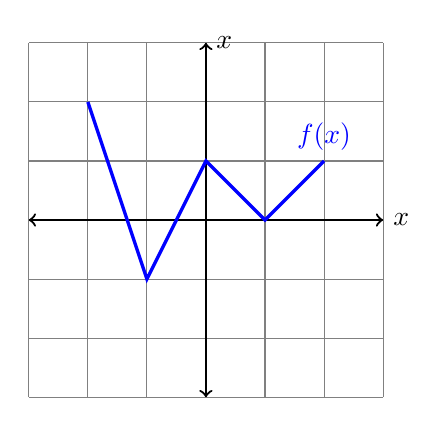
\begin{tikzpicture}[scale=\scl]
            \draw[color=gray] (-3,-3) grid (3,3);
            \draw[thick, black, <->] (-3,0) -- (3,0) node[anchor=west]{$x$};
            \draw[thick, black, <->] (0,-3) -- (0,3) node[anchor=west]{$x$};
            \draw[very thick, blue] (-2,2) -- (-1,-1) -- (0,1) -- (1,0) -- (2,1)
            node[anchor=south]{$f(x)$}; 
        \end{tikzpicture} 
        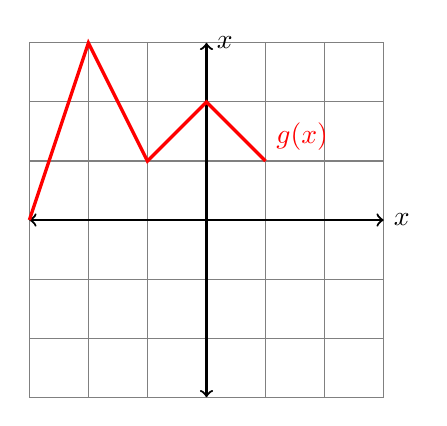
\begin{tikzpicture}[scale=\scl]
            \draw[color=gray] (-3,-3) grid (3,3);
            \draw[thick, black, <->] (-3,0) -- (3,0) node[anchor=west]{$x$};
            \draw[thick, black, <->] (0,-3) -- (0,3) node[anchor=west]{$x$};
            \draw[very thick, red] (-3,0) -- (-2,3) -- (-1,1) -- (0,2) -- (1,1)
            node[anchor=south west]{$g(x)$}; 
        \end{tikzpicture}
    \end{center}
\begin{exerciseSolution}
\end{exerciseSolution}

\item Use the function below to plot \\
    (a) $f(x)-3$, \quad (b) $f(x+1)$, \quad (c) $\frac{1}{2}f(x)$, \quad (d) $-f(x)$,
    \quad and (e) $\frac{1}{f(x)}$. 
    \begin{center}
        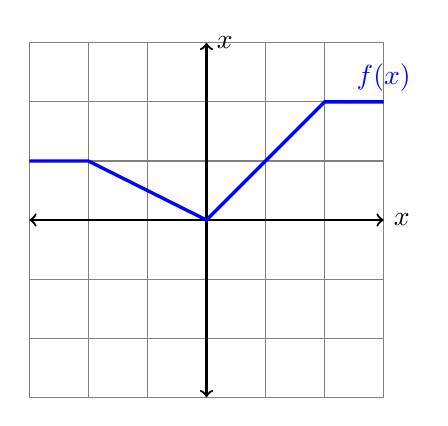
\begin{tikzpicture}[scale=\scl]
            \draw[color=gray] (-3,-3) grid (3,3);
            \draw[thick, black, <->] (-3,0) -- (3,0) node[anchor=west]{$x$};
            \draw[thick, black, <->] (0,-3) -- (0,3) node[anchor=west]{$x$};
            \draw[very thick, blue] (-3,1) -- (-2,1) -- (0,0) -- (2,2) -- (3,2)
            node[anchor=south]{$f(x)$}; 
        \end{tikzpicture} 
        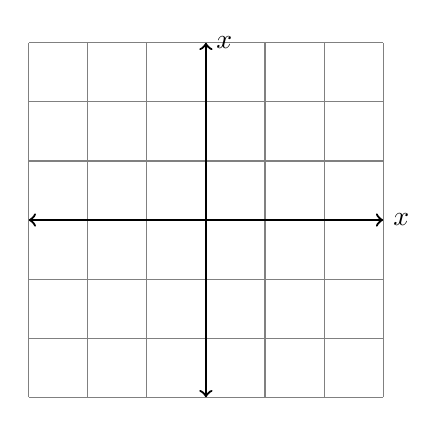
\begin{tikzpicture}[scale=\scl]
            \draw[color=gray] (-3,-3) grid (3,3);
            \draw[thick, black, <->] (-3,0) -- (3,0) node[anchor=west]{$x$};
            \draw[thick, black, <->] (0,-3) -- (0,3) node[anchor=west]{$x$};
        \end{tikzpicture}
    \end{center}
\begin{exerciseSolution}
\end{exerciseSolution}


\end{exercises}
\afterexercises



\clearpage
